\chapter{Das Photon im Standardmodell der Teilchenphysik}
\setcounter{section}{8}
\setcounter{subsection}{0}
\setcounter{subsubsection}{1}
\setcounter{secnumdepth}{3}
% Boxen-Stile definieren
\tcbset{physikbox/.style={colback=blue!5!white, colframe=blue!75!black, fonttitle=\bfseries}}
\tcbset{mathebox/.style={colback=green!5!white, colframe=green!50!black, fonttitle=\bfseries}}
\tcbset{didaktikbox/.style={colback=yellow!5!white, colframe=yellow!50!black, fonttitle=\bfseries}}
\tcbset{hypobox/.style={colback=orange!5!white, colframe=orange!75!black, fonttitle=\bfseries}}
\tcbset{hinweisbox/.style={colback=gray!10!white, colframe=black!40!black, fonttitle=\bfseries}}

\subsection{Das Standardmodell: Überblick}

Das \textbf{Standardmodell der Teilchenphysik}\index{Standardmodell der Teilchenphysik} ist eine erfolgreiche Theorie, die die bekannten fundamentalen Teilchen und ihre Wechselwirkungen – mit Ausnahme der \textbf{Gravitation}\index{Gravitation} – beschreibt.  
Es kombiniert die \textbf{Quantenelektrodynamik (QED)}\index{Quantenelektrodynamik (QED)}, die \textbf{Quantentheorie der schwachen Wechselwirkung}\index{Schwache Wechselwirkung} und die \textbf{Quantenchromodynamik (QCD)}\index{Quantenchromodynamik (QCD)} zu einem konsistenten Rahmenwerk.

Die fundamentalen Bausteine sind \textbf{Fermionen}\index{Fermion}, die Materie bilden, und \textbf{Bosonen}\index{Boson}, die als Austauschteilchen für die fundamentalen Kräfte wirken.  
Bosonen sind Teilchen mit ganzzahligem Spin, die durch ihre Austauschwirkung die fundamentalen Kräfte vermitteln.  
Zu den Eichbosonen\index{Eichboson} zählen das \textbf{Photon}\index{Photon} (Träger der elektromagnetischen Wechselwirkung), die \textbf{$W^\pm$- und $Z^0$-Bosonen}\index{W-Boson}\index{Z-Boson} (Träger der schwachen Wechselwirkung) sowie die \textbf{Gluonen}\index{Gluon} (Träger der starken Wechselwirkung).  
Das \textbf{Higgs-Boson}\index{Higgs-Boson} spielt eine besondere Rolle: Es verleiht den Elementarteilchen über den \textbf{Higgs-Mechanismus}\index{Higgs-Mechanismus} ihre Masse.

Die Wechselwirkungen werden durch \textbf{Eichsymmetrien}\index{Eichsymmetrie} beschrieben, die in der mathematischen Sprache von \textbf{Lie-Gruppen}\index{Lie-Gruppe} formuliert sind.  
Das Standardmodell basiert auf der Symmetriegruppe \(\mathrm{SU(3)} \times \mathrm{SU(2)} \times \mathrm{U(1)}\)\index{SU(3)}\index{SU(2)}\index{U(1)}.  
Jeder dieser Faktoren steht für eine fundamentale Wechselwirkung:  
\(\mathrm{SU(3)}\) für die starke Wechselwirkung, \(\mathrm{SU(2)} \times \mathrm{U(1)}\) für die \textbf{elektroschwache Theorie}\index{Elektroschwache Theorie}.

Trotz seines Erfolges ist das Standardmodell unvollständig:  
Es erklärt weder die Gravitation, noch liefert es Antworten auf Fragen nach \textbf{Dunkler Materie}\index{Dunkle Materie} oder \textbf{Dunkler Energie}\index{Dunkle Energie}.

\subsection{U(1)-Eichsymmetrie und das Photon}



Die elektromagnetische Wechselwirkung lässt sich elegant als \textbf{U(1)-Eich\-symmetrie}\index{U(1)-Eichsymmetrie} formulieren.  
Die Gruppe \(\mathrm{U(1)}\)\index{U(1)} ist die Menge aller komplexen Zahlen mit Betrag 1, die sich in der Form \(e^{i\theta}\) darstellen lassen.  
Sie ist eine \textbf{abelsche Gruppe}\index{Abelsche Gruppe}, d.\,h. die Gruppenoperation (hier: Multiplikation) ist kommutativ.  
In der Sprache der Mathematik gehört \(\mathrm{U(1)}\) zu den \textbf{Lie-Gruppen}\index{Lie-Gruppe}, also zu stetigen Symmetriegruppen, deren Elemente durch stetige Parameter beschrieben werden.

In der Quantenmechanik beschreibt eine \textbf{globale U(1)-Symmetrie}\index{Globale Symmetrie} die Invarianz der Wellenfunktion unter einer Phasenänderung \(\psi \to e^{i\alpha}\psi\).  
Nach dem \textbf{Noether-Theorem}\index{Noether-Theorem} ist diese Symmetrie direkt mit der \textbf{Ladungserhaltung}\index{Ladungserhaltung} verknüpft.

Wird die Symmetrie \emph{lokal} gemacht – d.\,h. der Phasenwinkel \(\alpha\) darf von Raum und Zeit abhängen –, spricht man von einer \textbf{lokalen U(1)-Eichsymmetrie}\index{Lokale Symmetrie}.  
Damit diese Invarianz erhalten bleibt, muss ein neues Feld eingeführt werden: das elektromagnetische Potential \(A_\mu\)\index{Elektromagnetisches Potential}.  
Dieses Feld kompensiert die Änderungen der Phase und führt zur \textbf{Eichkopplung}\index{Eichkopplung} zwischen geladenen Teilchen und dem Feld.

Die Quantisierung dieses Feldes liefert das \textbf{Photon}\index{Photon} als masseloses \textbf{Eichboson}\index{Eichboson} der elektromagnetischen Wechselwirkung.  
Seine Eigenschaften – insbesondere Masselosigkeit und Spin 1 – folgen direkt aus der Struktur der U(1)-Symmetrie.

Die U(1)-Eichtheorie ist ein Spezialfall einer abelschen Eichtheorie\index{Abelsche Eichtheorie} und bildet den elektromagnetischen Sektor der \textbf{elektroschwachen Theorie}\index{Elektroschwache Theorie}.  
Ihre mathematische Einfachheit macht sie zu einem idealen Ausgangspunkt, um komplexere Theorien wie \(\mathrm{SU(2)}\) oder \(\mathrm{SU(3)}\) zu verstehen.
\vspace{1em}
\begin{tcolorbox}[didaktikbox, title=U(1) anschaulich erklärt]
	\label{box:u1_kreis}
	\small
	\begin{minipage}{0.35\textwidth}
		\centering
		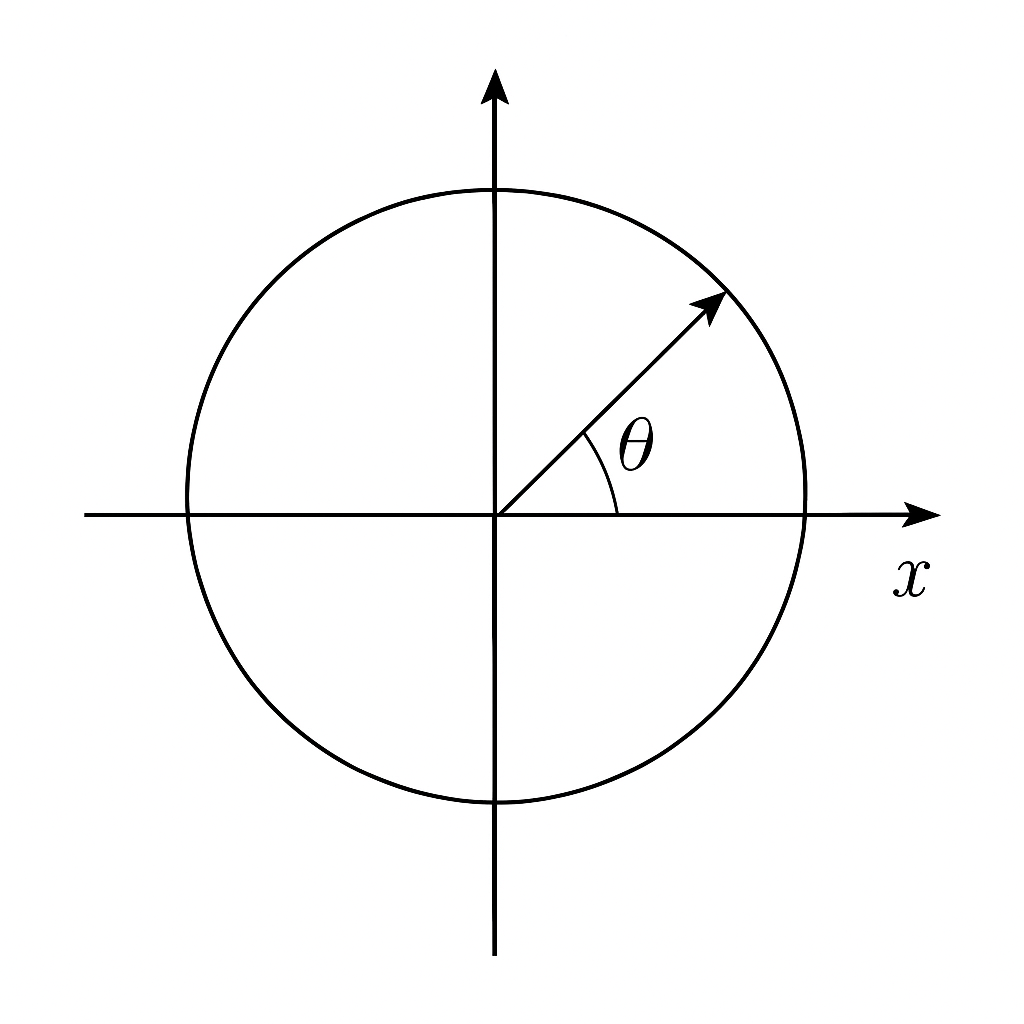
\includegraphics[width=\linewidth]{bilder/u1_kreis.png}
	\end{minipage}%
	\begin{minipage}{0.63\textwidth}
		Die Gruppe \(\mathrm{U(1)}\) kann man sich anschaulich als alle möglichen
		Drehungen auf einem Kreis vorstellen.  
		Jeder Punkt auf dem Kreis wird durch einen Winkel \(\theta\) beschrieben.  
		In der Quantenmechanik entspricht dies einer Phasenänderung der Wellenfunktion
		– der Abstand zum Ursprung bleibt immer gleich, nur die Richtung ändert sich.
	\end{minipage}
\end{tcolorbox}

\subsection{Elektroschwache Vereinheitlichung}


Die \textbf{elektroschwache Theorie}\index{Elektroschwache Theorie} beschreibt die Vereinigung der \textbf{elektromagnetischen Wechselwirkung}\index{Elektromagnetische Wechselwirkung} und der \textbf{schwachen Wechselwirkung}\index{Schwache Wechselwirkung} in einem gemeinsamen theoretischen Rahmen.  
Sie wurde Ende der 1960er Jahre von \textbf{Sheldon Glashow}\index{Glashow, Sheldon}, \textbf{Abdus Salam}\index{Salam, Abdus} und \textbf{Steven Weinberg}\index{Weinberg, Steven} entwickelt und bildet einen zentralen Bestandteil des \textbf{Standardmodells der Teilchenphysik}\index{Standardmodell der Teilchenphysik}.  
Für diese Leistung erhielten sie 1979 den \textbf{Nobelpreis für Physik}\index{Nobelpreis für Physik}.

Mathematisch basiert die elektroschwache Theorie auf der Symmetriegruppe \(\mathrm{SU(2)} \times \mathrm{U(1)}\)\index{SU(2)}\index{U(1)}.  
Die \(\mathrm{SU(2)}\)-Symmetrie beschreibt die schwache Wechselwirkung mit ihren drei Eichbosonen \(W^1, W^2, W^3\)\index{Eichboson}, während die \(\mathrm{U(1)}\)-Symmetrie den elektromagnetischen Anteil repräsentiert.  
Durch eine Mischung (\emph{Weinberg-Winkel}\index{Weinberg-Winkel}) der Felder \(W^3\) und \(B\) (dem U(1)-Boson) entstehen das masselose \textbf{Photon}\index{Photon} und das neutrale \textbf{\(Z^0\)-Boson}\index{Z-Boson}.

Die elektroschwache Symmetrie wird durch den \textbf{Higgs-Mechanismus}\index{Higgs-Mechanismus} spontan gebrochen.  
Dadurch erhalten die \(W^\pm\)- und \(Z^0\)-Bosonen\index{W-Boson}\index{Z-Boson} eine Masse, während das Photon masselos bleibt.  
Diese Eigenschaft ist ein direkter Ausdruck der verbleibenden ungebrochenen U(1)-Symmetrie\index{U(1)-Eichsymmetrie} der Elektrodynamik.

Die experimentelle Bestätigung der elektroschwachen Theorie gelang Anfang der 1980er Jahre am CERN\index{CERN} durch den direkten Nachweis der \(W\)- und \(Z\)-Bosonen.  
Diese Entdeckung gilt als einer der größten Erfolge der modernen Teilchenphysik.
\vspace{1em}
\begin{tcolorbox}[didaktikbox, title=Vom \(W^3\) und \(B\) zum Photon]
	\label{box:weinberg_mischung}
	\small
	\begin{minipage}{0.35\textwidth}
		\centering
		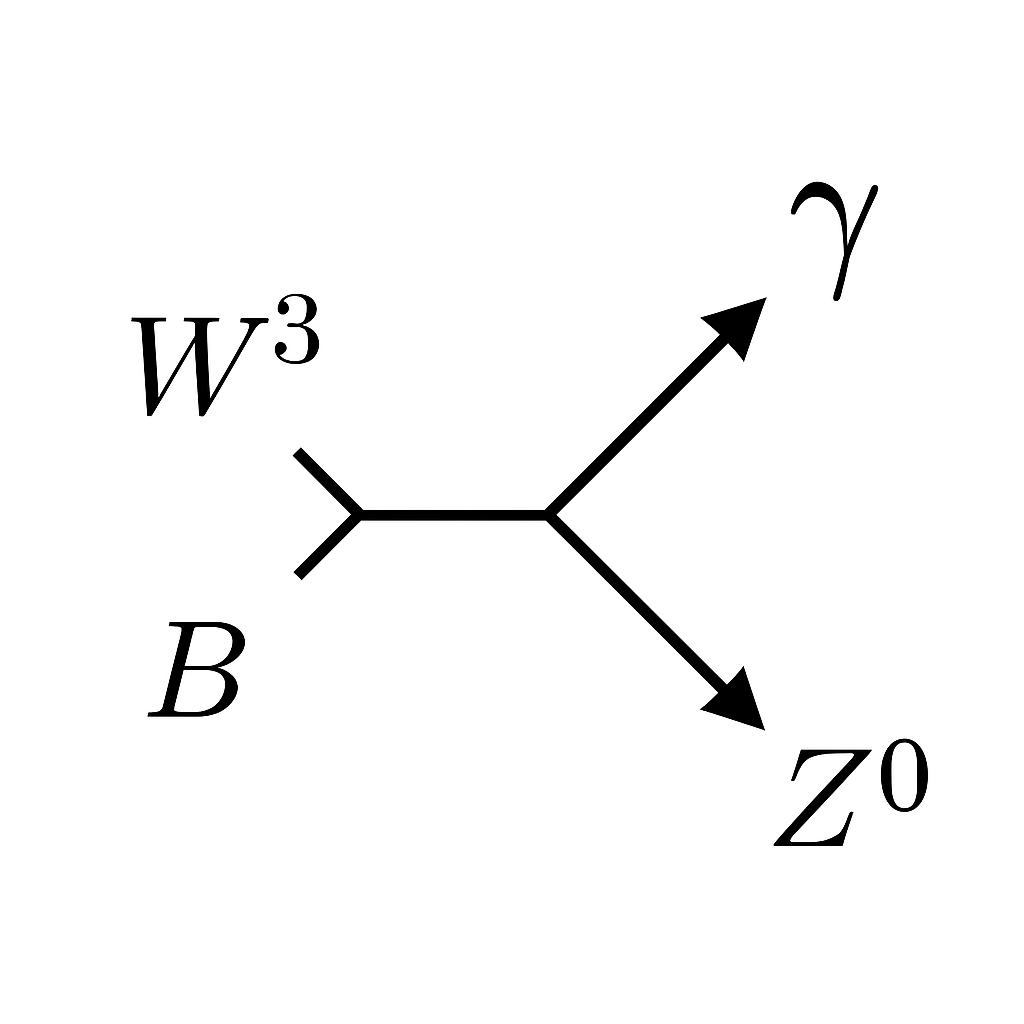
\includegraphics[width=\linewidth]{bilder/weinberg_mischung.png}
	\end{minipage}%
	\begin{minipage}{0.63\textwidth}
		In der elektroschwachen Theorie entstehen das \textbf{Photon} \(\gamma\) und das neutrale 
		\(\mathbf{Z^0}\)-Boson durch eine Mischung der Felder \(W^3\) und \(B\) 
		– beschrieben durch den \textbf{Weinberg-Winkel} \(\theta_W\).  
		\vspace{0.3em}
		
		Mathematisch gilt:
		\[
		\begin{aligned}
			\gamma &= \phantom{-}\cos\theta_W \, B + \sin\theta_W \, W^3 \\
			Z^0    &= -\sin\theta_W \, B + \cos\theta_W \, W^3
		\end{aligned}
		\]
		Diese Rotation der Felder erklärt, warum das Photon masselos bleibt, während 
		das \(Z^0\)-Boson eine Masse erhält.
	\end{minipage}
\end{tcolorbox}


\subsection{Warum ist das Photon masselos?}


Das \textbf{Photon}\index{Photon} ist im Rahmen des \textbf{Standardmodells der Teilchenphysik}\index{Standardmodell der Teilchenphysik} ein masseloses \textbf{Eichboson}\index{Eichboson} der elektromagnetischen Wechselwirkung.  
Seine Masselosigkeit ist eine direkte Folge der ungebrochenen \textbf{U(1)-Eichsymmetrie}\index{U(1)-Eichsymmetrie} in der \textbf{Quantenelektrodynamik (QED)}\index{Quantenelektrodynamik (QED)}.

Im \textbf{Higgs-Mechanismus}\index{Higgs-Mechanismus}, der in der elektroschwachen Theorie die \(W^\pm\)- und \(Z^0\)-Bosonen\index{W-Boson}\index{Z-Boson} mit Masse versieht, bleibt genau eine Eichsymmetrie ungebrochen: die U(1)-Symmetrie der Elektrodynamik.  
Das zugehörige Eichfeld wird als Photon identifiziert – und da ungebrochene Eichsymmetrien immer zu masselosen Austauschteilchen führen, besitzt das Photon keine Ruhemasse.

Mathematisch äußert sich dies darin, dass in der Lagrangedichte\index{Lagrangedichte} des elektromagnetischen Feldes kein Massenterm der Form \(\frac{1}{2} m^2 A_\mu A^\mu\) auftritt.  
Ein solcher Term würde die Eichinvarianz verletzen und ist daher verboten.

Die experimentellen Grenzen für eine eventuelle Photonenmasse sind extrem streng:  
Messungen setzen eine obere Schranke von weniger als \(10^{-18}\,\mathrm{eV}/c^2\)\index{Photonenmasse} fest.  
Praktisch ist das Photon daher perfekt masselos – eine Eigenschaft, die für die unendliche Reichweite\index{Reichweite elektromagnetischer Wechselwirkung} der elektromagnetischen Kraft entscheidend ist.
\vspace{1em}
\begin{tcolorbox}[hinweisbox, title=Masselosigkeit und Reichweite]
	\label{box:reichweite_masselos}
	\small
	Die Reichweite einer fundamentalen Wechselwirkung hängt direkt von der Masse ihres Austauschteilchens ab.  
	\begin{itemize}
		\item \textbf{Masselose Austauschteilchen} (z.\,B. Photonen) vermitteln Kräfte mit unbegrenzter Reichweite.  
		\item \textbf{Massive Austauschteilchen} (z.\,B. \(W^\pm\)- und \(Z^0\)-Bosonen) vermitteln Kräfte mit endlicher Reichweite, die durch die \emph{Compton-Wellenlänge} \(\lambda_C = \hbar/(mc)\) bestimmt wird.
	\end{itemize}
	Für das Photon folgt aus seiner Masselosigkeit die unendliche Reichweite der elektromagnetischen Wechselwirkung.
\end{tcolorbox}
\vspace{1em}
\begin{tcolorbox}[physikbox, title=Masseloses Photon und Spinwirkung über große Distanzen]
	\label{box:photon_spin_reichweite}
	\small
	Ein masseloses Photon besitzt keine Reichweitenbegrenzung für die Vermittlung seiner quantisierten Eigenschaften.  
	Das hat zwei wesentliche Konsequenzen:
	\begin{itemize}
		\item \textbf{Unendliche Reichweite der Wechselwirkung:} Die elektromagnetische Kraft wirkt prinzipiell über beliebige Entfernungen.
		\item \textbf{Erhalt der Spinrichtung (Polarisation):} Da das Photon masselos ist und sich mit Lichtgeschwindigkeit bewegt, bleibt seine Spin- bzw. Polarisationsausrichtung auch über kosmologische Distanzen erhalten. 
	\end{itemize}
	In verschränkten Quantenzuständen bedeutet dies, dass die Korrelation der Polarisation zweier Photonen selbst dann messbar bleibt, wenn sie weit voneinander entfernt sind – eine Folge der Kombination von Masselosigkeit und quantenmechanischer Verschränkung.
\end{tcolorbox}


\subsection{Vergleich mit anderen Eichbosonen}

Im \textbf{Standardmodell der Teilchenphysik}\index{Standardmodell der Teilchenphysik} existieren mehrere \textbf{Eichbosonen}\index{Eichboson}, die fundamentale Wechselwirkungen vermitteln.  
Das \textbf{Photon}\index{Photon} unterscheidet sich von ihnen in wesentlichen Eigenschaften:

\begin{itemize}
	\item \textbf{Photon (QED):} Masselos, Spin \(1\), vermittelt die \textbf{elektromagnetische Wechselwirkung}\index{Elektromagnetische Wechselwirkung}.  
	Reichweite: unendlich.
	
	\item \(\mathbf{W^\pm}\)- und \(\mathbf{Z^0}\)-\textbf{Bosonen} (elektroschwache Theorie)\index{W-Boson}\index{Z-Boson}:  
	Spin \(1\), besitzen hohe Masse (\(\approx 80{-}91\,\mathrm{GeV}/c^2\)), Reichweite: etwa \(10^{-18}\,\mathrm{m}\).  
	Vermitteln die \textbf{schwache Wechselwirkung}\index{Schwache Wechselwirkung}.
	
	\item \textbf{Gluonen} (QCD)\index{Gluon}:  
	Spin \(1\), formal masselos, vermitteln die \textbf{starke Wechselwirkung}\index{Starke Wechselwirkung}.  
	Reichweite jedoch effektiv stark begrenzt durch \textbf{Confinement}\index{Confinement} – Gluonen treten nicht als freie Teilchen auf.
	
	\item \textbf{Graviton}\index{Graviton} (hypothetisch):  
	Spin \(2\), masselos, würde die Gravitation vermitteln.  
	Noch nicht experimentell nachgewiesen.
\end{itemize}

Der entscheidende Unterschied:  
Nur das Photon tritt als frei messbares, masseloses Austauschteilchen mit unbegrenzter Reichweite auf.  
W- und Z-Bosonen sind massiv und daher kurzreichweitig, Gluonen sind zwar masselos, aber durch Confinement in gebundenen Zuständen gefangen.
\vspace{1em}
\begin{tcolorbox}[hinweisbox, title=Vergleich der Eichbosonen]
	\label{box:eichbosonen_vergleich}
	\small
	
	\resizebox{\linewidth}{!}{%
		\begin{tabular}{lcccc}
			\textbf{Teilchen} & \textbf{Spin} & \textbf{Masse} & \textbf{Reichweite} & \textbf{Wechselwirkung} \\
			\hline
			Photon & 1 & 0 & unendlich & elektromagnetisch \\
			\(W^\pm\) & 1 & \(\approx 80\,\mathrm{GeV}/c^2\) & \(10^{-18}\,\mathrm{m}\) & schwach \\
			\(Z^0\) & 1 & \(\approx 91\,\mathrm{GeV}/c^2\) & \(10^{-18}\,\mathrm{m}\) & schwach \\
			Gluon & 1 & 0 & \emph{effektiv kurz} & stark (Confinement) \\
			Graviton (hyp.) & 2 & 0 & unendlich & Gravitation \\
		\end{tabular}%
	}
	
\end{tcolorbox}




\subsection{Offene Fragen und Erweiterungen}

Trotz des Erfolgs des \textbf{Standardmodells der Teilchenphysik}\index{Standardmodell der Teilchenphysik} bleiben zentrale Fragen unbeantwortet, die auch das \textbf{Photon}\index{Photon} betreffen oder seinen theoretischen Rahmen erweitern könnten:

\begin{itemize}
	\item \textbf{Photonenmasse}\index{Photonenmasse}:  
	Experimentell gilt das Photon als masselos, doch ist nicht ausgeschlossen, dass es eine extrem kleine, bislang unmessbare Masse besitzt.  
	Verbesserte Messungen könnten diese Grenze weiter einschränken oder – überraschend – eine endliche Masse nachweisen.
	
	\item \textbf{Wechselwirkung mit Dunkler Materie}\index{Dunkle Materie}:  
	Ob Photonen in irgendeiner Form mit Dunkler Materie koppeln, ist unbekannt.  
	Direkte und indirekte Suchmethoden könnten hier in Zukunft Hinweise liefern.
	
	\item \textbf{Vereinheitlichte Theorien}\index{Vereinheitlichte Theorie}:  
	In Theorien jenseits des Standardmodells – etwa \textbf{Große Vereinheitlichung (GUT)}\index{Große Vereinheitlichung} oder \textbf{String\-theorien}\index{Stringtheorie} – ist das Photon Teil eines größeren Symmetriegefüges.  
	Diese Modelle könnten neue Eigenschaften oder Partnerteilchen vorhersagen.
	
	\item \textbf{Quantengravitation}\index{Quantengravitation}:  
	Eine konsistente Theorie, die die Gravitation mit den Quantenfeldern der Teilchenphysik verbindet, fehlt bislang.  
	Die Wechselwirkung des Photons mit hypothetischen \textbf{Gravitonen}\index{Graviton} oder der Struktur der Raumzeit auf kleinster Skala ist weitgehend unerforscht.
	
	\item \textbf{Neue Symmetrien oder Teilchen}:  
	Erweiterungen des Standardmodells könnten zusätzliche Eichbosonen oder Symmetrien beinhalten, die Einfluss auf die Rolle des Photons haben.
\end{itemize}

Die Beantwortung dieser Fragen erfordert eine Kombination aus präzisen Experimenten, neuen Beobachtungstechnologien und theoretischen Durchbrüchen.  
Das Photon bleibt damit nicht nur ein zentrales Werkzeug der Physik, sondern auch ein Schlüssel zu möglichen neuen physikalischen Welten.
\subsection{Fazit}
\subsubsection*{Das Photon – Teilchen, Welle und Fenster zur Zukunft}
\phantomsection
Das \textbf{Photon}\index{Photon} hat in der Geschichte der Physik eine einzigartige Rolle gespielt:  
Es war der Schlüssel zur Entstehung der Quantentheorie, der Ausgangspunkt für die Entwicklung der \textbf{Quantenelektrodynamik (QED)}\index{Quantenelektrodynamik (QED)} und bleibt bis heute ein unverzichtbares Werkzeug der experimentellen und theoretischen Forschung.

Vom \textbf{Photoeffekt}\index{Photoeffekt} über die \textbf{Compton-Streuung}\index{Compton-Streuung} bis hin zu modernen Anwendungen wie \textbf{Quantenkommunikation}\index{Quantenkommunikation} und \textbf{Photonik}\index{Photonik} hat das Photon nicht nur unsere physikalischen Modelle geprägt, sondern auch Technologien ermöglicht, die unseren Alltag verändern.

Im Rahmen des \textbf{Standardmodells der Teilchenphysik}\index{Standardmodell der Teilchenphysik} steht das Photon für eine ungebrochene \textbf{U(1)-Eichsymmetrie}\index{U(1)-Eichsymmetrie} – eine mathematische Eleganz, die sich in seiner Masselosigkeit und unendlichen Reichweite widerspiegelt.  
Gleichzeitig zeigt der Blick auf offene Fragen, dass wir vom vollständigen Verständnis noch weit entfernt sind.
\newpage
\noindent
Das Photon verbindet fundamentale Eigenschaften der Natur:
\begin{itemize}
	\item \textbf{Welle und Teilchen} in einer einzigen Quantenbeschreibung.
	\item \textbf{Masseloser Bote} mit unendlicher Reichweite.
	\item \textbf{Präzise Messsonde} in Astronomie, Teilchenphysik und Quantenoptik.
	\item \textbf{Schlüsselakteur} in künftigen Technologien wie Quantencomputern und photonischen Schaltkreisen.
\end{itemize}

Seine Doppelrolle als theoretisches Fundament und praktisches Werkzeug macht das Photon zu einem der faszinierendsten Objekte der Physik.  
Es ist nicht nur ein Bestandteil unseres physikalischen Weltbildes, sondern auch ein Tor zu noch unbekannten Aspekten des Universums – ein Tor, das wir in den kommenden Jahrzehnten weiter aufstoßen werden.



Auch wenn das Photon im Standardmodell in einer klaren und konsistenten Rolle erscheint, 
bleibt es zugleich ein Symbol für die Grenzen dieser Theorie.  
Um diese Doppelfunktion hervorzuheben – als Fundament und als Brücke zu neuer Physik – 
fassen wir die wichtigsten Erkenntnisse didaktisch zusammen und werfen anschließend 
einen spekulativen Blick in die Zukunft.
\vspace{1em}
\begin{tcolorbox}[didaktikbox, title=Didaktischer Abschluss: Das Photon im Standardmodell]
	\label{box:didaktik_kapVIII}
	Das Photon ist nicht nur ein Werkzeug der Quantenoptik und modernen Technologie, 
	sondern auch eine Schlüsselfigur im theoretischen Fundament der Physik.  
	
	\medskip
	\textbf{Kernbotschaft:}  
	Seine Rolle als masseloses Eichboson der ungebrochenen U(1)-Symmetrie verbindet mathematische Eleganz, 
	experimentelle Präzision und kosmische Reichweite.  
	Damit steht das Photon exemplarisch für die Stärke – aber auch für die Grenzen – des Standardmodells.
\end{tcolorbox}
\vspace{1em}
\begin{tcolorbox}[hypobox, title={Was wäre, wenn das Standardmodell nur ein Zwischenschritt wäre?}]
	\label{Merksatz zum Photon}
	Ein Gedankenspiel:
	\begin{itemize}
		\item Wenn Photonen mit Dunkler Materie wechselwirken könnten, würde das unser Verständnis von Kosmologie revolutionieren.  
		\item Ein Nachweis winziger Photonenmassen würde die Struktur der Elektrodynamik grundlegend ändern.  
		\item Neue Symmetrien oder verborgene Partnerteilchen des Photons könnten in einer erweiterten Theorie jenseits des Standardmodells auftauchen.  
		\item Vielleicht ist das Photon sogar der Schlüssel zur Verbindung von Quantenfeldtheorie und Gravitation.  
	\end{itemize}
	
	\medskip
	Solche spekulativen Perspektiven führen über das Standardmodell hinaus – und öffnen die Tür 
	zu einem künftigen Kapitel über \emph{neue Physik}.
\end{tcolorbox}
